\chapter{Implementation}
\label{cha:implementation}

This chapter is going through some of the implementation details throughout the development of the project.

\section{Interfacing with Emotiv}
The Unity 3D plugin package from Emotiv comes in a suite of 11 C\# files which we will describe in a bit more detail. In order to get access to this data, an  \texttt{EPOCManager} object was created. This object contains all the plugins in the package apart from  \texttt{EdkDll}, \texttt{EmoState}, \texttt{EmoProfileManagement} and \texttt{LabelDraw}. In the following subsections, I am going to provide some very short code snippets since these might prove useful in the future for someone wishing to develop using Unity and Emotiv.

\subsection{EdkDll}
Contains the implementation of the Emotiv API.

\subsection{EmoAffectiv} 
This class gives access to the player emotions described in section \ref{part:affectiv} through calls by directly accessing one of the public instance variables. For example,

\begin{Verbatim}[frame=single, framesep=3mm, label={[Beginning of code]End of code}]
EmoAffectiv.frustrationScore
\end{Verbatim}

returns a value representing how frustrated the user is.

In the game, frustration is used to get the rain started once the level is percentage is higher than 50\%. 

\subsection{EmoCognitiv} 
It is a class containing methods to start or reset the training. It automatically handles events which start, reset, erase, declare successful or failed training. I have added accessor methods to obtain the current action, its power and the trained actions. I have also added a GUI method, \texttt{DoTrainingCompleteAction(int windowID)} which pops up the window asking the user whether the training should be accepted or rejected and it handles the response appropriately. Before starting the training though, the 4 actions (push, pull, left, right) have to be activated through a call such as: 

\begin{Verbatim}[frame=single, framesep=3mm, label={[Beginning of code]End of code}]
EmoCognitiv.EnableCognitivAction(EmoCognitiv.cognitivActionList[6], 
				true);
\end{Verbatim}
		
where 6 represents the index of \textit{right} action. At the end, the list of 4 actions has to be set through a call to 

\begin{Verbatim}[frame=single, framesep=3mm, label={[Beginning of code]End of code}]
EmoCognitiv.EnableCognitivActionsList();
\end{Verbatim}

The skill for the \textit{push} action is obtained as follows:

\begin{Verbatim}[frame=single, framesep=3mm, label={[Beginning of code]End of code}]
Single pushSkill = EmoEngine.Instance.CognitivGetActionSkillRating(
			(uint)EmoUserManagement.currentUser,
			EmoCognitiv.cognitivActionList[1]); 
\end{Verbatim}

\subsection{EmoEngine}
`Is the logical abstraction of the functionality that Emotiv provides in edk.dll.'\cite{emotivSDKUserManual}

\subsection{EmoEngineInst}
It is used most often to change the connection method from live data to simulated data (through the use of EmoComposer (subsection \ref{part:emocomposer})).

\subsection{EmoExpressiv}
The EmoExpressiv class is obtained to get access to the player's facial expressions through simple calls to the public instance variables, such as the following which checks whether the player did a left wink:

\begin{Verbatim}[frame=single, framesep=3mm, label={[Beginning of code]End of code}]
EmoExpressiv.isLeftWink
\end{Verbatim}

In CogniDriver, left wink is used to change the camera view. Clenching teeth will action the car's handbrake. 

\subsection{EmoGyroData}
Gives access to the head position in relation to the circle observed in figure. One may also obtained the \texttt{x} and \texttt{y} coordinates of the gyro. However, I could not find the maximum and minimum values, nor are there 2 online references which give the same numbers.

\subsection{EmoProfileManagement}
This class is useful to handle the player profiles. In CogniDriver, I have limited the number of player profiles to 10 because of the following reasons:
\begin{itemize}
	\item The training for a saved profile can take a few MB;
	\item Unity does not contain a drop down list as a GUI element;
	\item Unity does not allow overflow of windows.
\end{itemize}

When the game starts, the list of user profiles (files saved with the \texttt{.up} extension) is loaded through a call to:

\begin{Verbatim}[frame=single, framesep=3mm, label={[Beginning of code]End of code}]
EmoProfileManagement.Instance.LoadProfilesFromFile();
\end{Verbatim}

A new profile is added by calling:

\begin{Verbatim}[frame=single, framesep=3mm, label={[Beginning of code]End of code}]
EmoProfileManagement.Instance.AddNewProfile(playerName);
\end{Verbatim}

Profile data is saved after training by a call to 

\begin{Verbatim}[frame=single, framesep=3mm, label={[Beginning of code]End of code}]
EmoProfileManagement.Instance.SaveCurrentProfile();
\end{Verbatim}

followed by

\begin{Verbatim}[frame=single, framesep=3mm, label={[Beginning of code]End of code}]
EmoProfileManagement.Instance.SaveProfilesToFile();
\end{Verbatim}

On selection of a profile, this is set by calling

\begin{Verbatim}[frame=single, framesep=3mm, label={[Beginning of code]End of code}]
EmoProfileManagement.Instance.SetUserProfile(selectedPlayer);
\end{Verbatim}

A profile is delete by calling

\begin{Verbatim}[frame=single, framesep=3mm, label={[Beginning of code]End of code}]
EmoProfileManagement.Instance.DeleteProfile(selectedPlayer);
\end{Verbatim}

\subsection{EmoState}
Represents the emotional status of the user at a given time \cite{emotivSDKUserManual}. This class is used by \texttt{EmoAffectiv}, \texttt{EmoExpressiv} and \texttt{EmoCognitiv} mainly. I did not need to call any functions directly from this class.

\subsection{EmoUserManagement}
Keeps track of the current user, the current number of user profiles and also fires events when adding or deleting a user. I did not need to use this class directly apart from obtaining the current user by calling

\begin{Verbatim}[frame=single, framesep=3mm, label={[Beginning of code]End of code}]
EmoUserManagement.currentUser
\end{Verbatim}

\subsection{LabelDraw}
I did not need to use this class while developing CogniDriver.

\subsection{Gyro mode}
Playing the game while using the headset's gyroscope is doable for forward/backward actions. However, most of the times the user is getting eyes off the screen meaning they may not see where and how the car is moving. 

\section{Scene description}
In Unity, a scene contains all the objects for a part of the game such as a level or a different screen. For CogniDriver, I have split the game in 6 scenes. All of the scenes, apart from the splash screen, will display the sensor contact quality, current action and the power of the current action. This can be observed in figure.

See figure \ref{fig:sceneInteraction} for an example of how the scenes interact with each other.

\begin{figure}
  \centering
  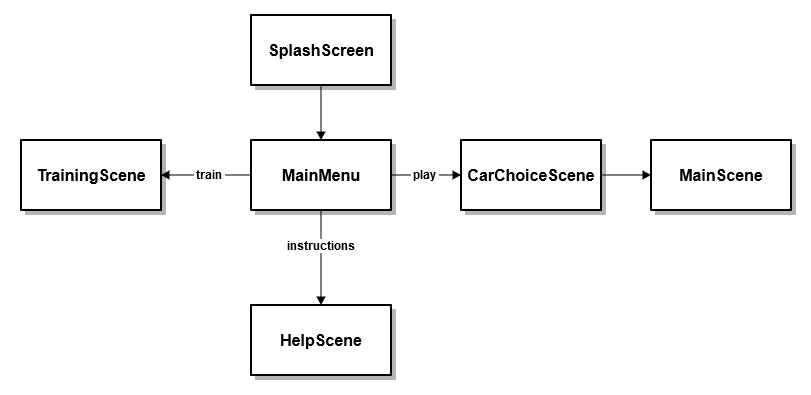
\includegraphics[width=450px]{sceneInteraction.png}
  \caption{Scene interaction diagram from the moment the application starts loading.}
    \label{fig:sceneInteraction}           
\end{figure}

\subsection{CarChoiceScene}
The purpose of this scene is to allow the player to choose a car model and colour. At the moment, I have only used 2 car models. I had three of them in mind but one of the models did not allow me to modify the grouping of its components. 

\subsection{HelpScene}
It is simple instructions describing how the game is to be played. Figure shows an example of how the instructions are displayed to the player.

\subsection{MainMenu}
This scene allows the player to:
\begin{itemize}
	\item manage the player profiles;
	\item start the race;
	\item train a player profile to be played in Cognitiv mode;
	\item see the highscores for Keyboard and Cognitiv mode in \textit{Statistics} tab;
	\item read instructions about training and playing the game;
	\item adjust the sound effects and music volume, fullscreen enabling and select the play mode;
	\item exit the game.
\end{itemize}

Figure shows an example of how the main menu scene looks like.

\subsection{MainScene}
This is the proper game play where the player is controlling the car around the track. 

\subsection{SplashScreen}
This represents the image the player is presented with during the initial loading of the game. The used image can be observed in figure.

\subsection{TrainingScene}
Its aim is to provide a place where the player can train the 5 actions: neutral (staying relaxed), push, pull, left, right. The training may also be reset for each action in turn. The user will receive visual feedback from the animated car on how well the training has been done. A screenshot can be observed in figure.

\section{Interesting aspects of development}

I took the decision of having the Cognitiv training done inside the game so that a new player would not need to open another application, for example the Emotiv Control Panel, in order to train the profile.

For passing variables between different scenes, Unity's \texttt{PlayerPrefs} module has been very useful. One example of its use is in saving the highscores. 
